\chapter{开发工具介绍}
\section{开发环境}
\label{sec:environment}
操作系统:Windows 10

开发工具:VS code

后端支持:Nodejs

框架支持:Angular 5

数据库:MySQL
\section{开发工具VS code}
\label{sec:vsCode}
VSCode是微软出的一款轻量级代码编辑器,免费而且功能强大,对JavaScript和NodeJS的支持非常好,自带很多功能,例如代码格式化,代码智能提示补全、Emmet插件等。它其实就是一款简单的代码编辑工具,跟Visual Studio、WebStorm、Eclipse、myEclipse...这些集成的开发环境并不是一个概念。但是它拥有极其强大的扩展性,只要安装对应的语言插件,就可以对该语言提供强大的支持。因此,选择这个开发工具能极大提高开发效率。
\section{依赖包管理}
\label{sec:dependencies_manage}
本应用选择npm(Node Package Manager)来对依赖包进行管理,NPM是随同NodeJS一起安装的包管理工具,能解决NodeJS代码部署上的很多问题,常见的功能有:
\begin{itemize}
	\item 允许用户从NPM服务器下载别人编写的第三方包到本地使用。
	\item 允许用户从NPM服务器下载并安装别人编写的命令行程序到本地使用。
	\item 允许用户将自己编写的包或命令行程序上传到NPM服务器供别人使用。
\end{itemize}
因为本应用需要使用nodejs部署服务器,所以无需其他的包管理器,直接可以使用npm进行包管理,我们只需要在package.json文件上配置所需的依赖,然后`npm install`即可安装所需的依赖包

\section{框架}
\label{sec:frame}
框架(Framework)是整个或部分系统的可重用设计,表现为一组抽象构件及构件实例间交互的方法;另一种定义认为,框架是可被应用开发者定制的应用骨架。前者是从应用方面而后者是从目的方面给出的定义。 

可以说,一个框架是一个可复用的设计构件,它规定了应用的体系结构,阐明了整个设计、协作构件之间的依赖关系、责任分配和控制流程,表现为一组抽象类以及其实例之间协作的方法,它为构件复用提供了上下文(Context)关系。因此构件库的大规模重用也需要框架。
 
构件领域框架方法在很大程度上借鉴了硬件技术发展的成就,它是构件技术、软件体系结构研究和应用软件开发三者发展结合的产物。在很多情况下,框架通常以构件库的形式出现,但构件库只是框架的一个重要部分。框架的关键还在于框架内对象间的交互模式和控制流模式。

框架比构件可定制性强。在某种程度上,将构件和框架看成两个不同但彼此协作的技术或许更好。框架为构件提供重用的环境,为构件处理错误、交换数据及激活操作提供了标准的方法。 

应用框架的概念也很简单。它并不是包含构件应用程序的 小片程序,而是实现了某应用领域通用完备功能(除去特殊应用的部分)的底层服务。使用这种框架的编程人员可以在一个通用功能已经实现的基础上开始具体的系 统开发。框架提供了所有应用期望的默认行为的类集合。具体的应用通过重写子类(该子类属于框架的默认行为)或组装对象来支持应用专用的行为。 

软件系统发展到今天已经很复杂了,特别是服务器端软件,设计到的知识,内容,问题太多。在某些方面使用别人成熟的框架,就相当于让别人帮你完成一些基 础工作,你只需要集中精力完成系统的业务逻辑设计。而且框架一般是成熟,稳健的,他可以处理系统很多细节问题,比如,事物处理,安全性,数据流控制等问 题。还有框架一般都经过很多人使用,所以结构很好,所以扩展性也很好,而且它是不断升级的,你可以直接享受别人升级代码带来的好处。 

\begin{figure}[h]
	\centering
	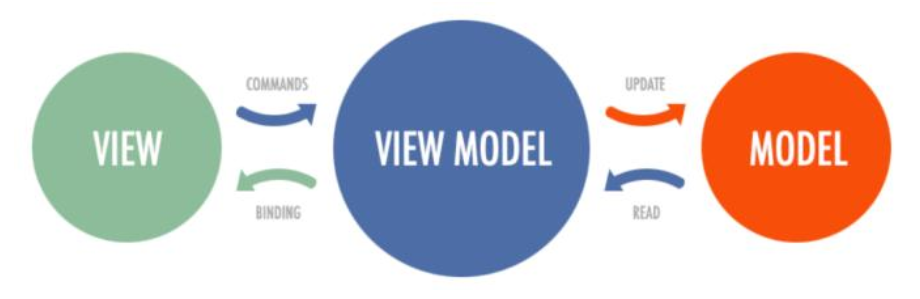
\includegraphics[width=0.5\textwidth]{image/mvvm.png}
	\caption{MVVM框架}
	\label{fig:mvvm}
\end{figure}
本应用使用的是2017年 11月1日 Google公司发布的Angular 5。angular\cite{Angular}作为当前最主流的三大前端框架之一,拥有及其完善的功能,而选择它的很重要的一个原因是,相比于vue和react这种轻量级的框架,它更适用于开发大型的,比较复杂的的企业级应用,它拥有完善的项目搭建脚手架,单元测试工具,这对于工程化,规范化的应用开发是十分有利的。
同时,它的可扩展性很强,需要新增什么功能,就新建一个组件,只要将组件导入项目中即可,无需在项目中改动过多的代码
当然,随着版本的更迭,angular也不断吸收vue,react等优秀框架的特点,不断改进自己,使得开发人员使用起来更加方便和得心应手。

使用方法:npm install -g @angular/cli

\section{后端服务器}
\label{sec:server}
后端服务器使用express + nodejs搭建

Node.js\cite{Nodejs} 是一个基于Chrome JavaScript 运行时建立的一个平台,简单的说它就是运行在服务端的 JavaScript。Node.js是一个事件驱动I/O服务端JavaScript环境,基于Google的V8引擎,V8引擎执行Javascript的速度非常快,性能非常好。Javascript是一个事件驱动语言,Node利用了这个优点,编写出可扩展性高的服务器。Node采用了一个称为“事件循环(event loop)”的架构,使得编写可扩展性高的服务器变得既容易又安全。提高服务器性能的技巧有多种多样。Node选择了一种既能提高性能,又能减低开发复杂度的架构。这是一个非常重要的特性。并发编程通常很复杂且布满地雷。Node绕过了这些,但仍提供很好的性能。

Node采用一系列“非阻塞”库来支持事件循环的方式。本质上就是为文件系统、数据库之类的资源提供接口。向文件系统发送一个请求时,无需等待硬盘(寻址并检索文件),硬盘准备好的时候非阻塞接口会通知Node。该模型以可扩展的方式简化了对慢资源的访问, 直观,易懂。Node.js使用Module模块去划分不同的功能,以简化应用的开发。Modules模块有点像C++语言中的类库。每一个Node.js的类库都包含了十分丰富的各类函数,比如http模块就包含了和http功能相关的很多函数,可以帮助开发者很容易地对比如http,tcp/udp等进行操作,还可以很容易的创建http和tcp/udp的服务器。

在几年的时间里,Node.JS逐渐发展成一个成熟的开发平台,吸引了许多开发者。有许多大型高流量网站都采用Node.JS进行开发,此外,开发人员还可以使用它来开发一些快速移动Web框架。除了Web应用外,NodeJS也被应用在许多方面,这些项目涉及到应用程序监控、媒体流、远程控制、桌面和移动应用等等。

Express 是一个基于 Node.js 平台的极简、灵活的 web 应用开发框架,它提供一系列强大的特性,帮助你创建各种 Web 和移动设备应用,使用 Express 可以快速地搭建一个完整功能的网站。

Express 框架核心特性如下:
\begin{itemize}
	\item 可以设置中间件来响应 HTTP 请求。
	\item 定义了路由表用于执行不同的 HTTP 请求动作。
	\item 可以通过向模板传递参数来动态渲染 HTML 页面。
\end{itemize}

\section{数据库}
\label{sec:database}
数据库(Database)是按照数据结构来组织、存储和管理数据的建立在计算机存储设备上的仓库\cite{XU}。简单来说是本身可视为电子化的文件柜——存储电子文件的处所,用户可以对文件中的数据进行新增、截取、更新、删除等操作。严格来说,数据库是长期储存在计算机内、有组织的、可共享的数据集合。数据库中的数据指的是以一定的数据模型组织、描述和储存在一起、具有尽可能小的冗余度、较高的数据独立性和易扩展性的特点并可在一定范围内为多个用户共享\cite{wdb}。

数据库有以下几个特点\cite{db}:
\begin{itemize}
	\item 实现数据共享

	数据共享包含所有用户可同时存取数据库中的数据,也包括用户可以用各种方式通过接口使用数据库,并提供数据共享。
	\item 减少数据的冗余度
	
	同文件系统相比,由于数据库实现了数据共享,因而避免了用户各自建立应用文件。从而,减少了大量重复数据,减少了数据冗余,维护了数据一致性。
	\item 数据的独立性
	
	数据的独立性,包括逻辑独立性和物理独立性。
	
	逻辑独立性,是指数据库中数据的逻辑结构与用户的应用程序是相互独立的。数据的逻辑结构改变了,用户的应用程序可以不变。
	
	物理独立性,是指数据库中数据的物理结构的变化不影响数据的逻辑结构。
	
	\item 数据实现集中控制
	
	在文件管理方式中,数据处于一种分散的状态,不同的用户或同一用户在不同处理中其文件之间毫无关系。
	利用数据库可对数据进行集中控制和管理,并通过数据结构(数据模型)表示各种数据的组织以及数据间的联系。
	
	\item 数据一致性和可维护性,以确保数据的安全性和可靠性
	
	\begin{itemize}
		\item 安全性控制:以防止数据丢失、错误更新和越权使用;
		\item 完整性控制:保证数据的正确性、有效性和相容性;
		\item 并发控制:使在同一时间周期内,允许对数据实现多路(多用户)存取,又能防止用户之间的不正常交互作用。
	\end{itemize}
	\item 故障恢复
	
	由数据库管理系统提供一套方法,可及时发现故障和修复故障,从而防止数据被破坏。数据库系统能尽快恢复数据库系统运行时出现的故障,可能是物理上或是逻辑上的错误。比如对系统的误操作造成的数据错误等。
\end{itemize}
就目前而言,数据库分为关系型(传统型)数据库和非关系型数据库。当前主流的关系型数据库有Oracle、DB2、Microsoft SQL Server、Microsoft Access、MySQL等。非关系型数据库有 NoSql、Cloudant。

两者各有其优缺点,非关系型数据库简单易部署,成本低,查询速度较快,利于数据分割,储存格式是key,value形式、文档形式、图片形式等等,所以可以存储基础类型以及对象或者是集合等各种格式\cite{oodb};而传统的关系型数据库相比于前者,可以做到更加复杂的数据查询,如多表联合查询等,而且其对事务的支持使得对于安全性能很高的数据访问要求得以实现。

由于关系型数据库的各个表之间存在的较强的联系,因此不利于数据的分散,也就是难以将数据分割存储到不同的服务器中,这会导致在数据量太大的时候对服务器的负荷加大。

